\section{Конструкторская часть}

В данном разделе рассматриваются этапы проектирования базы данных, спроектированы триггер и функция.

\subsection{Формализация сущностей системы}

На основе выделенных ранее сущностей \ref{fig:anal:use-case} спроектированны таблицы 
базы данных.

\subsubsection{Таблица Visitor}

Содержит информцию о посетителях мазазинов, которые включает следующие поля:

\begin{enumerate}[label=\arabic*.]
    \item id --- индетификатор пользователя, который является первичным ключом;
    \item description --- описание пользователя, вещественный тип;
    \item location --- положение пользователя на плане магазина, символьный тип 
    который состои из двух вещественных чисел;
    \item view --- вектор взгляда, символьный тип, состоящий из шести вещественных
    чисел, которые задают вектор взгляда;
    \item detection --- описание пользователя, символьный тип, 
    состоящий из 4 вещественных
    чисел, которые задают прямоугольник обнуружения посетителя.
\end{enumerate}

\subsubsection{Таблица Camera}

Содержит информацию о камерах в магазине, которые включает следующая поля:

\begin{enumerate}[label=\arabic*.]
    \item id --- номер камеры в магазине, первичный ключ;
    \item location --- положение пользователя на плане магазина, символьный тип 
    который состои из трех вещественных чисел;
    \item resolution --- разрешение камеры, символьный тип состоящий из двух
    вещественных чисел;
    \item rotation --- наклон камеры, символьный тип. Является матрицей
    состоящих из 9 вещественных чисел;
    \item type --- тип камеры, символьный тип.
\end{enumerate}

\subsubsection{Таблица Shelf}

Содержит информацию о полках в магазине, которые включает следующая поля:

\begin{enumerate}[label=\arabic*.]
    \item id --- номер полки в магазине, первичный ключ;
    \item location --- положение пользователя на плане магазина, символьный тип 
    который состои из трех вещественных чисел;
    \item length --- длина полки, вещественный тип.
\end{enumerate}

\subsubsection{Таблица Product}

Содержит информацию о товарах в магазине, которые включает следующая поля:

\begin{enumerate}[label=\arabic*.]
    \item id --- номер товара в магазине, первичный ключ;
    \item location --- положение товара на плане магазина, символьный тип 
    который состои из трех вещественных чисел;
    \item name --- имя товара, символьный тип;
    \item dataEnd --- срок годности, тип дата;
    \item weight --- вес товара, вещественный тип;
    \item status --- статус товара, целочисленный тип;
    \item price --- цена товара, вещественный тип.
\end{enumerate}

\subsubsection{Таблица ChainStore}

Содержит информацию о сетях магазинов, которые включает следующая поля:

\begin{enumerate}[label=\arabic*.]
    \item id --- номер магазина, первичный ключ;
    \item location --- положение магазина в городе, символьный тип 
    который состои из двух вещественных чисел (широта и долгота);
    \item name --- имя магазина, символьный тип;
    \item nameDir --- имя директора магазина, символьный тип;
    \item income --- доход магазина, вещественный тип;
    \item consumption --- расходы магазина, вещественный тип.
\end{enumerate}

На рисунке \ref{fig:cons:ER} предствалена ER диаграмма база данных.

\begin{figure}[ht!]
	\centering
	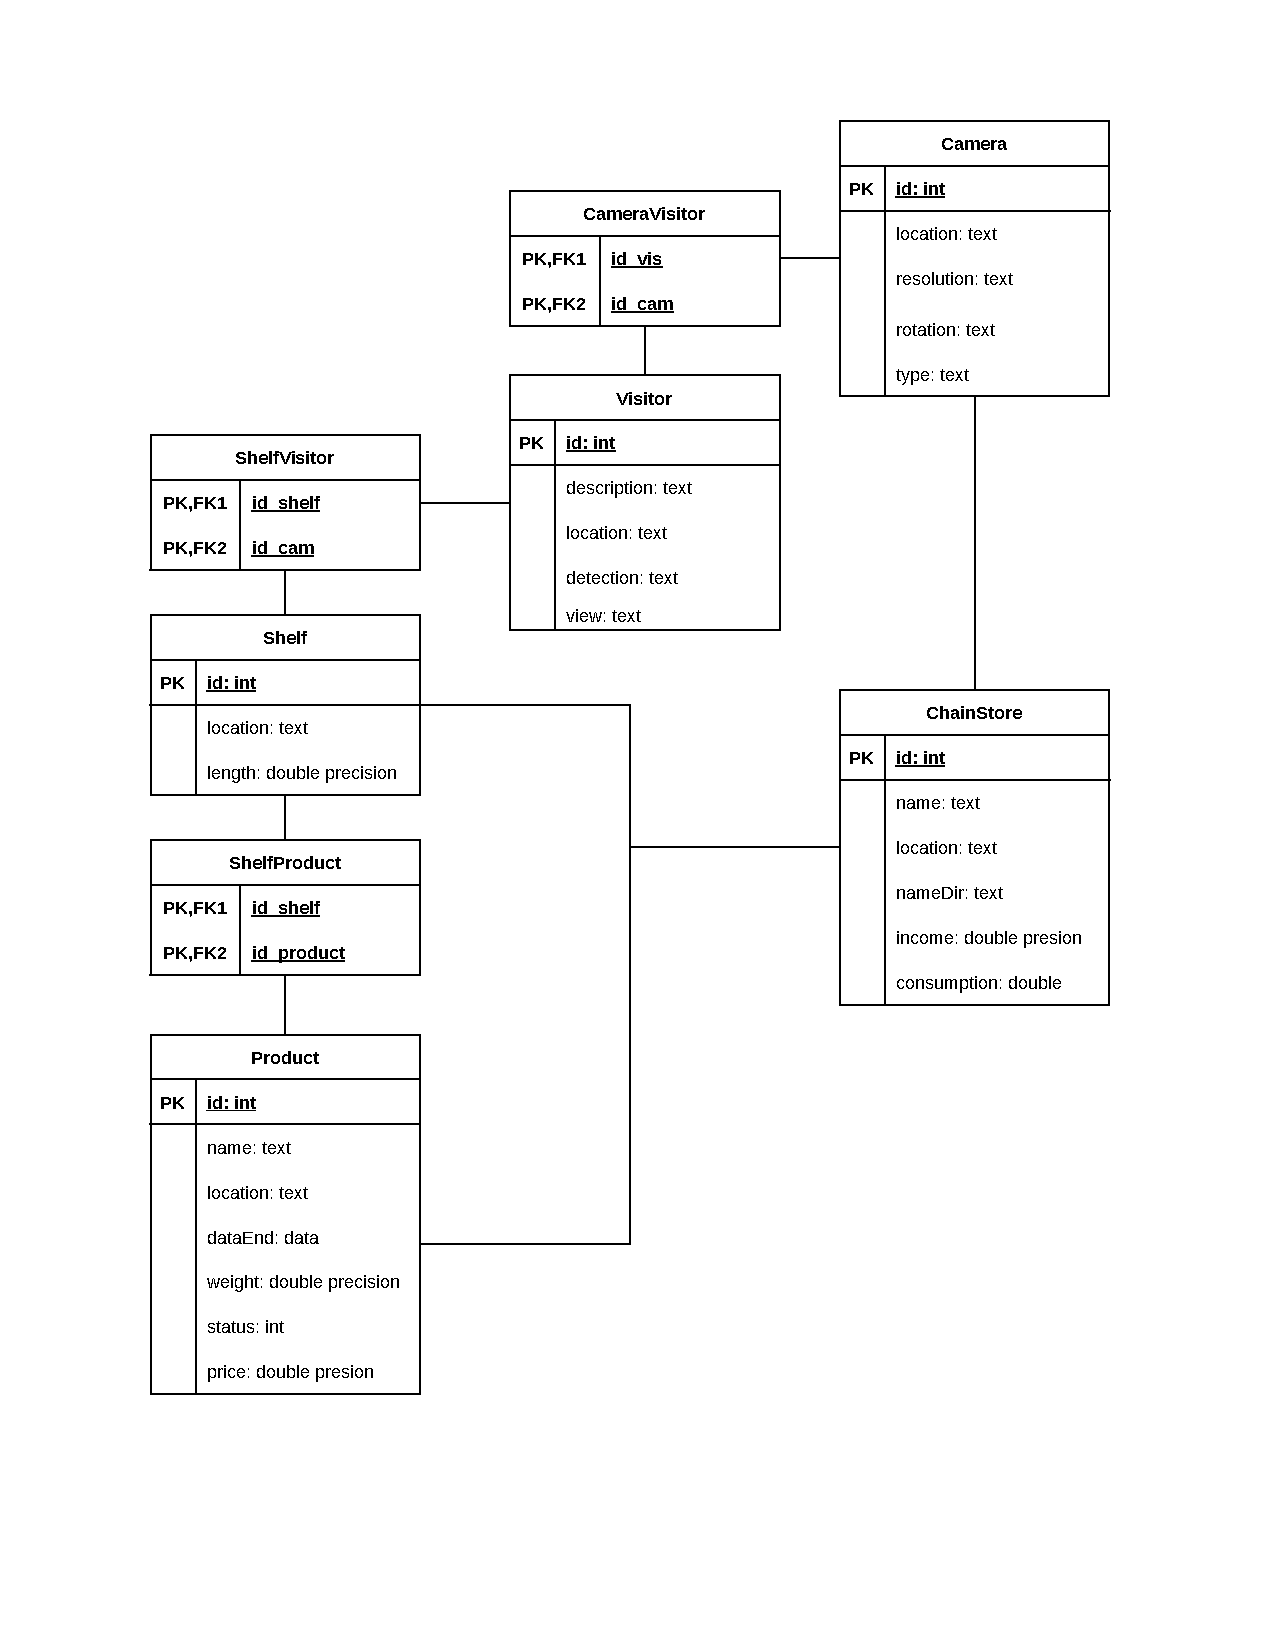
\includegraphics[width=1\linewidth]{assets/images/ER-diagram.drawio.pdf}
	\caption{Use-case диаграмма}
	\label{fig:cons:ER}
\end{figure}
\FloatBarrier

\subsection{Ролевая модель}

Для обеспечения работы пользователей с сисетмой управления базами данных, выделена
следующая ролевая модель.

\subsubsection{Сотрудник Employee}

\begin{enumerate}[label=\arabic*.]
    \item SELECT --- над таблицей Visitor.
\end{enumerate}


\subsubsection{Охрана Security}

\begin{enumerate}[label=\arabic*.]
    \item SELECT --- над таблицей Visitor;
    \item SELECT --- над таблицами Camera, Product, Shelf.
\end{enumerate}


\subsubsection{Администратор Administrator}

\begin{enumerate}[label=\arabic*.]
    \item все права над таблицами Visitor;
    \item все права над таблицами Camera, Product, Shelf;
    \item все права над таблицами ChainStore.
\end{enumerate}

Ролевая модель на уровне СУБД позволяет обеспечить безопасное управление данными.

\subsection{Разработка триггера и функции}

В СУБД предусмотрена функция, которая проверяет местоположение пользователя относительно выхода. 
Данная функция возращает статус посетителя (находится внутри или вне магазина).

Также системе представлен ALTER триггер, который оповщает систему о том, 
что посетитель вышел из магазина.



\subsection*{Вывод}

В данном разделе были формализированны сущности системы, представлен рисунок диаграммы сущности системы,
выделены ролевые модели, спроектированы триггер и функция.